%% This is file `elsarticle-template-1-num.tex',
%%
%% Copyright 2009 Elsevier Ltd
%%
%% This file is part of the 'Elsarticle Bundle'.
%% ---------------------------------------------
%%
%% It may be distributed under the conditions of the LaTeX Project Public
%% License, either version 1.2 of this license or (at your option) any
%% later version.  The latest version of this license is in
%%    http://www.latex-project.org/lppl.txt
%% and version 1.2 or later is part of all distributions of LaTeX
%% version 1999/12/01 or later.
%%
%% Template article for Elsevier's document class `elsarticle'
%% with numbered style bibliographic references
%%
%% $Id: elsarticle-template-1-num.tex 149 2009-10-08 05:01:15Z rishi $
%% $URL: http://lenova.river-valley.com/svn/elsbst/trunk/elsarticle-template-1-num.tex $
%%
\documentclass[preprint,12pt]{elsarticle}
\setcounter{secnumdepth}{0}
\usepackage{xcolor}
\usepackage{rotating}
\usepackage{sectsty}
\usepackage{graphicx}
\usepackage{amsmath,amssymb}
\usepackage{adjustbox}
\usepackage{fancyhdr}
\usepackage{float}
\usepackage{multirow}
\usepackage{amsmath,amsthm,amssymb,amsfonts,float,graphicx}
\usepackage{hyperref}
\linespread{1.2}
\usepackage[margin=1in]{geometry}
\usepackage{hyperref}
\usepackage[margin=1in]{geometry}
\usepackage{subcaption}
\usepackage[demo]{graphicx}
\usepackage{titlesec}

\titleformat{\section}[hang]{\large\bf}{\textup{\thesubsection}}{1em}{}[]

\titleformat{\subsection}[hang]{\normalfont\normalsize\bfseries}{\textup{\thesubsection}}{1em}{}[]

\titleformat{\subsubsection}[hang]{\normalfont\normalsize\bfseries}{\thesubsubsection}{1em}{}


%% natbib.sty is loaded by default. However, natbib options can be
%% provided with \biboptions{...} command. Following options are
%% valid:

%%   round  -  round parentheses are used (default)
%%   square -  square brackets are used   [option]
%%   curly  -  curly braces are used      {option}
%%   angle  -  angle brackets are used    <option>
%%   semicolon  -  multiple citations separated by semi-colon
%%   colon  - same as semicolon, an earlier confusion
%%   comma  -  separated by comma
%%   numbers-  selects numerical citations
%%   super  -  numerical citations as superscripts
%%   sort   -  sorts multiple citations according to order in ref. list
%%   sort&compress   -  like sort, but also compresses numerical citations
%%   compress - compresses without sorting
%%
%% \biboptions{comma,round}

% \biboptions{}

\journal{Journal Name}

\begin{document}

\begin{frontmatter}

%% Title, authors and addresses

\title{A Neural Network Based Algorithm for Dynamically Adjusting Activity Targets to Sustain Exercise Engagement Among People Using Activity Trackers}

%% use the tnoteref command within \title for footnotes;
%% use the tnotetext command for the associated footnote;
%% use the fnref command within \author or \address for footnotes;
%% use the fntext command for the associated footnote;
%% use the corref command within \author for corresponding author footnotes;
%% use the cortext command for the associated footnote;
%% use the ead command for the email address,
%% and the form \ead[url] for the home page:
%%
%% \title{Title\tnoteref{label1}}
%% \tnotetext[label1]{}
%% \author{Name\corref{cor1}\fnref{label2}}
%% \ead{email address}
%% \ead[url]{home page}
%% \fntext[label2]{}
%% \cortext[cor1]{}
%% \address{Address\fnref{label3}}
%% \fntext[label3]{}


%% use optional labels to link authors explicitly to addresses:
%% \author[label1,label2]{<author name>}
%% \address[label1]{<address>}
%% \address[label2]{<address>}

\author[1,2]{Ramin Mohammadi} 
\author[2]{Amanda Jayne Centi}
\author[2]{Mursal Atif}
\author[2,3,4]{Stephen Agboola}
\author[2,3,4]{Kamal Jethwani}  
\author[2,3,4]{Joseph C Kvedar}  
\author[1,2]{Sagar Kamarthi \corref{cor1}}

\address[1]{Department of Mechanical and Industrial Engineering, Northeastern University, Boston, United States}
\address[2]{Connected Health Innovation, Partners Healthcare, Boston, United States.}
\address[3]{Department of Dermatology, Massachusetts General Hospital, Boston, United States.}
\address[4]{Harvard Medical School, Harvard University, Boston, United States.}
\cortext[cor1]{sagar@coe.edu}

\begin{abstract}
%% Text of abstract
It is well established that lack of physical activity is detrimental to overall health of an individual. Modern day activity trackers enable individuals to monitor their daily activity to meet and maintain targets and to promote activity encouraging behavior. The benefits of activity trackers are offset by adherence that fades over time due to multifarious factors. One key method to improve adherence to goals, where goals form a motivation to improve on the historic performance metrics. In this work we develop a model to dynamically adjusted the activity target that can be realistically achieved by the activity tracker users. We consider user-specific personal, social, and environmental factors, daily step count through the current week (7 days), and an entropy measure that characterizes the pattern of daily step count for the week. The prediction model prescribes target activity for the forthcoming week based on the aforementioned inputs. Data for the study was collected for 30 participants over a duration of 9 weeks. The predicted target daily count using the prediction model closely matches with the actual average daily count of the week. The proposed work can be used to set personalized goals in accordance with the individual's level of activity.

\end{abstract}

\begin{keyword}
 Activity trackers \sep exercise engagement \sep dynamic activity targets \sep neural network \sep activity target prediction \sep machine learning.
%% keywords here, in the form: keyword \sep keyword

%% MSC codes here, in the form: \MSC code \sep code
%% or \MSC[2008] code \sep code (2000 is the default)

\end{keyword}

\end{frontmatter}


%%
%% Start line numbering here if you want
%%
\tableofcontents 
\section{Introduction}
Studies have reported the efficacy of physical activity in reducing the risk of disease. However, physical inactivity is on rise in the US population \cite{bassuk2005epidemiological}. Considering that physical inactivity was the fourth leading cause of mortality in 2016 \cite{mercer2016behavior}, there is much emphasis on developing methods to increase and maintain a healthy level of physical activity. Wearable fitness trackers enable individuals to monitor their activity levels and patterns to manage their health. Fitness tracker are expanding their commercial market owing to lower costs and enhanced efficiency \cite{eheman2012annual}. It was observed that about 20\% of the general health-tracking population uses smart devices such as medical devices, mobile phone apps, or online tools to track their health data \cite{michie2009effective}. The use of technology to objectively monitor physical activity is associated with higher levels of activity \cite{wang2016mobile}. However, the potential benefits derived from the use of physical activity trackers is challenged by the limited and transient adoption of these devices, which necessarily require sustained use to exert their intended effect. The continued engagement with fitness trackers is an issue that begs for further research \cite{wang2016mobile}.  
\par
Authors’ recent work [10] studies the factors associated with the adoption and sustained use of physical activity trackers. Previous studies have demonstrated that motivational factors are associated with physical activity level \cite{bassuk2005epidemiological}. Lack of time, fatigue and a dislike for exercise are some of the barriers that reflect a lack of motivation to engage in physical activity \cite{bassuk2005epidemiological}. It is reported that adjustment to targets for activity levels are likely to enhance the users’ commitment to physical activity and engagement with fitness trackers \cite{gouveia2015we}. With the rise of machine learning and availability of the activity tracker data, it is of interest to create a model for actively adjusting the weekly target. Machine learning techniques such as multiple linear regression and neural networks (NNs) have been applied for time series forecasting tasks. It is shown that NNs perform better than traditional models for time series forecasting \cite{hill1996neural}. NN’s are better at estimating a forecast for nonlinear time series with few assumption about the data \cite{hill1996neural}. Researchers have focused on variable/feature selection in many areas using expert knowledge, automatic dimension reduction methods and data visualization tools. The above mentioned methods might have their own biases which can lead to under performing classification results \cite{cheng2006feature}.

This study to our knowledge is the first of its kind to dynamically adjust the activity target for activity trackers. We use two approaches, mainly, data-driven approach and knowledge-based approach. First, for feature extraction we constructed explanatory variables using factor analysis then crated a Shannon entropy value for each participant per week. Next, We used random forest for variable selection over generated variables from previous step. We used the engineered features as an input to machine learning algorithms. We have developed two neural networks model namely data driven neural networks (DDNN) and knowledge based neural network (KBNN). Last we compared the developed model using 10-fold cross validation. Figure [\ref{fig:1}] shows the study flow diagram highlighting the key steps undertaken in the study.


\begin{figure}[H]
\centering\includegraphics[width=1\linewidth]{Flow_chart.png}
\caption{Study flow diagram} 
\label{fig:1}
\end{figure}

\section{Results}

We compare the performance of the two neural network models. Table [\ref{tab:Performance}] outlines the performance of DDNN and KBNN models. We observe that the data driven method performs better than the knowledge driven method in predicting the daily count of steps. The average RMSE value of data driven approach is less than the average RMSE value of the Knowledge driven approach [Figure \ref{fig:2}]. However this performance comes at a cost of interpretability. The factors generated as the features for the data driven approach are difficult to interpret. 

\begin{table}[H]
\centering
\caption{Performance of DDNN and KBNN models}
\begin{tabular}{lllllll}
\hline
Model & Variable Selection  & Performance Measure & Min.    & Max.    & Mean    & Median  \\
\hline
DDNN  & Random forest-based & RMSE                & 1505.00 & 1783.36 & 1922.54 & 2053.58 \\
KBNN  & Knowledge-based     & RMSE                & 1993.38 & 2307.50 & 2427.42 & 3000.05 \\
DDNN  & Random forest-based & R-Square            & 0.6127  & 0.6946  & 0.7355  & 0.7868  \\
KBNN  & Knowledge-based     & R-Square            & 0.0018  & 0.4629  & 0.5356  & 0.6445 \\
\hline
\label{tab:Performance}
\end{tabular}
\end{table}


\begin{figure}[H]
\centering\includegraphics[width=0.7\linewidth]{boxplot.png}
\caption{Box-Plots of RMSE for DDNN and KBNN models} 
\label{fig:2}
\end{figure}


Despite its difficulty we have retrieved the top 10 variables related to the final factors used in the DDNN model for learning purposes reported in Figure [\ref{fig:7}, \ref{fig:8}, \ref{fig:9}, \ref{fig:10}].  







\section{Discussion}
In this work we develop a machine learning model to predict the number of steps covered daily by an individual. We investigate two neural network models for the prediction problem. We observe that the NNs with data driven features (DDNN) performs better than the NNs with knowledge based features (KBNN). The first one yielded an average RMSE of 1922.54 steps while the later one yielded an average RMSE of 2427.42 steps. The variables of importance reported by DDNN model were different from the variables reported by KBNN model. The current study can be used the set goals for individuals accompanied by proper motivation that will improve the sustained use of the activity tracker \cite{couper2010engagement,bossen2013adherence,davies2012prospective}. Researchers showed that easy achieving goals may also lead to abandonment of the activity tracker. An overestimation of number of step counts will allow to set goals that will not be very easily achieved \cite{murnane2015mobile}. 


\color{red}

Add why this model will be useful or how it will be useful 

\color{black}
\section{Methods}

We inducted 30 (BMI 25 kg/m2 or greater) participants for the study. Over a period of 9 weeks, data related to daily steps was collected from the fitness tracker for each participant. Data from multiple questionnaires were collected for each participant. These questionaires are (Behavioral Regulation  in  Exercise  Questionnaire  (BREQ-2) \citep{markland2004modification}  and  Barriers  to  Being  Active  (BBA) \citep{BBA}),  a depression screening (Patient Health Questionnaire (PHQ-8) \citep{kroenke2009phq}), Prochaskas Stage of Change \citep{holmen2016stages},and general health questions (PROMIS Global-10) \citep{hays2009development}). The details of the questionnaires and hardware used for monitoring daily steps are explained in detail below. 

\subsection{Data Collection}
The data for building the machine learning model was generated from a 9-week, non-randomized pilot study. This study enrolled 30 male and female (9 male and 21 female) adults from a local MGH-affiliated clinic with a body mass index (BMI) of 25 kg/m2 or greater. After screening participants and seeking their consent, the research team directed the participants to the study website (\url{http://wellocracystudy.org}) to read through information regarding the study and the types and features of activity trackers they could choose for their use during the 9-week study. The study staff assisted the participants with the device set up process as needed. In the study 27 participants chose to use the FitBit Charge model, Two of them the FitBit One, and one of them chose the FitBit Zip. 

\par
Participants were instructed to continuously wear the activity tracker for the entire period of the study. The first week was treated as a run-in period. For the remaining weeks, the step goal for each participant was determined as 110\% of their respective average step count achieved in the first week. Participants were contacted minimally during the eight-week period to facilitate observation of participants’ activity-tracker habits without interference. 
\par
At the end of the study, participants completed a closeout survey either online or in paper format and underwent a phone interview to gather information on their experiences during the study. All interviews were conducted by a trained neuropsychologist and transcribed for analysis. Baseline and closeout questionnaires included questions about their technology use and ownership, thoughts about and perceived barriers to exercise and activity (BREQ-2 and BBA), a depression screening (PHQ-8), Prochaska’s Stage of Change, and PROMIS Global-10. The BREQ-2 is designed to gauge the extent to which reasons for exercise are internalized and self-determined based on the following categories: motivation, external, introjected, identified and intrinsic. In contrast, the BBA assess whether participants gauge certain categories as reasons for inactivity and include energy, willpower, time, resources, etc. For each category, a score of 5 or greater would indicate that category as a substantial barrier to a person’s ability to exercise. during the study 10 participants were removed from the study since they did not use the trackers. That left the study with 20 participants. The summary of the participants are given in the table below.

\begin{table}[H]
\begin{tabular}{|l|l|l|}
\hline
Variable                                   &                                          &              \\ \hline
Age, years (SD)                            &                                          & 48.9 (9.54)  \\ \hline
Male gender, n (\%)                        &                                          & 9 (30)       \\ \hline
\multirow{2}{*}{BMI at enrollment (SD)}    & Mean                                     & 32.48 (4.59) \\ \cline{2-3} 
                                           & Range                                    & 25-41.2      \\ \hline
\multirow{3}{*}{Race, n (\%)}              &                                          &              \\ \cline{2-3} 
                                           & White                                    & 21 (70)      \\ \cline{2-3} 
                                           & Non-White                                & 9 (30)       \\ \hline
\multirow{7}{*}{Marital status, n (\%)}    &                                          &              \\ \cline{2-3} 
                                           & Married                                  & 8 (26.7)     \\ \cline{2-3} 
                                           & Divorced/Separated                       & 8 (26.7)     \\ \cline{2-3} 
                                           & Single (never married)                   & 8 (26.7)     \\ \cline{2-3} 
                                           & Living with partner                      & 3 (10)       \\ \cline{2-3} 
                                           & Widowed                                  & 1 (3.3)      \\ \cline{2-3} 
                                           & No response                              & 2 (6.7)      \\ \hline
\multirow{8}{*}{Education, n (\%)}         &                                          &              \\ \cline{2-3} 
                                           & 12 years or completed high school or GED & 5 (16.7)     \\ \cline{2-3} 
                                           & Some college                             & 5 (16.7)     \\ \cline{2-3} 
                                           & College graduate                         & 9 (30)       \\ \cline{2-3} 
                                           & Post high school                         & 2 (6.7)      \\ \cline{2-3} 
                                           & Post Graduate                            & 2 (6.7)      \\ \cline{2-3} 
                                           & Less than high school                    & 3 (10)       \\ \cline{2-3} 
                                           & Unknown                                  & 4 (13.3)     \\ \hline
\multirow{7}{*}{Employment status, n (\%)} &                                          &              \\ \cline{2-3} 
                                           & Employed/self employed                   & 15 (50)      \\ \cline{2-3} 
                                           & Disabled                                 & 5 (16.7)     \\ \cline{2-3} 
                                           & Unemployed                               & 5 (16.7)     \\ \cline{2-3} 
                                           & Student                                  & 1 (3.3)      \\ \cline{2-3} 
                                           & Retired                                  & 1 (3.3)      \\ \cline{2-3} 
                                           & Unknown                                  & 3 (10)       \\ \hline
\end{tabular}
\end{table}

\subsubsection{Experimental Setting}
We randomly divide the data into training and test set using participant level. We choose 16 participants data as training dataset and remaining 5 participants dataset as test dataset. We perform all the experiments and tune hyper-parameters over training dataset only and test the models on the test dataset. 


\subsection{Feature Extraction and Variable Selection}

\par
 In the data-driven approach we consider all data from the questionnaires and  the daily step count data from the activity tracker. The baseline questionnaires generated 96 variables. We screened the variables to determine candidate predictors for building a machine learning model. In the first iteration of the variable screening process, 11 variables whose variance was zero were eliminated to reduce the feature dimensions. In the second iteration, pairwise correlations (Pearson correlation above 0.95) among the variables are examined to drop redundant variables. We did not drop any variables based on pairwise correlations because the correlations were not strong enough.
 

\begin{figure}[H]
\centering\includegraphics[width=0.5\linewidth]{NOn_graphical.png}
\caption{Comparison  of  the  determination  of  the  of  factors  to  retain  by  the  optimal  coordinates,  the  acceleration  factor,  the  parallel  analysis,  and  the  Keyser-Guttman rule.} 
\label{fig:3}
\end{figure}

\subsubsection{Factor Analysis}
Factor Analysis (FA) is an exploratory method aimed at finding underlying factors (set of variables) from which the observed variables were generated. A factor is a weighted average of the original variables, and FA is applied on the correlation matrix of the observed variables. In other words, FA is a statistical method used to describe variability among observed, correlated variables in terms of a potentially lower number of unobserved variables called factors.FA is a linear method which assumes that there are some unknown common factors which the observed variables are dependent on. The other goal of FA is to find factors and relation to reduce the dimensionality of the data \cite{fodor2002survey}. As a part of third iteration, We use FA to find out the uniqueness among the remaining observed variables \cite{thompson2007exploratory}.   We performed FA over the remaining 85 variables to identify latent factors that are a combination of observed variables. To count for correlation among the factors, oblique rotation is used to model factors as linear combination of observed variables. The FA yielded 18 latent factors with eigenvalues greater than mean [Figure \ref{fig:3}]. They together covered 99\% of the total variance in the data. These 18 latent factors are considered candidate predictors of target step count for the forthcoming week.


In addition to the features extracted from the questionnaires, we generate features from the daily step count which are aggregated on a weekly basis. We consider a 7-variable feature vector to represent the number of steps achieved for each day a week. The distribution of steps among all participants day-wise is shown in Figure \ref{fig:4}.


\begin{figure}[H]
\centering
  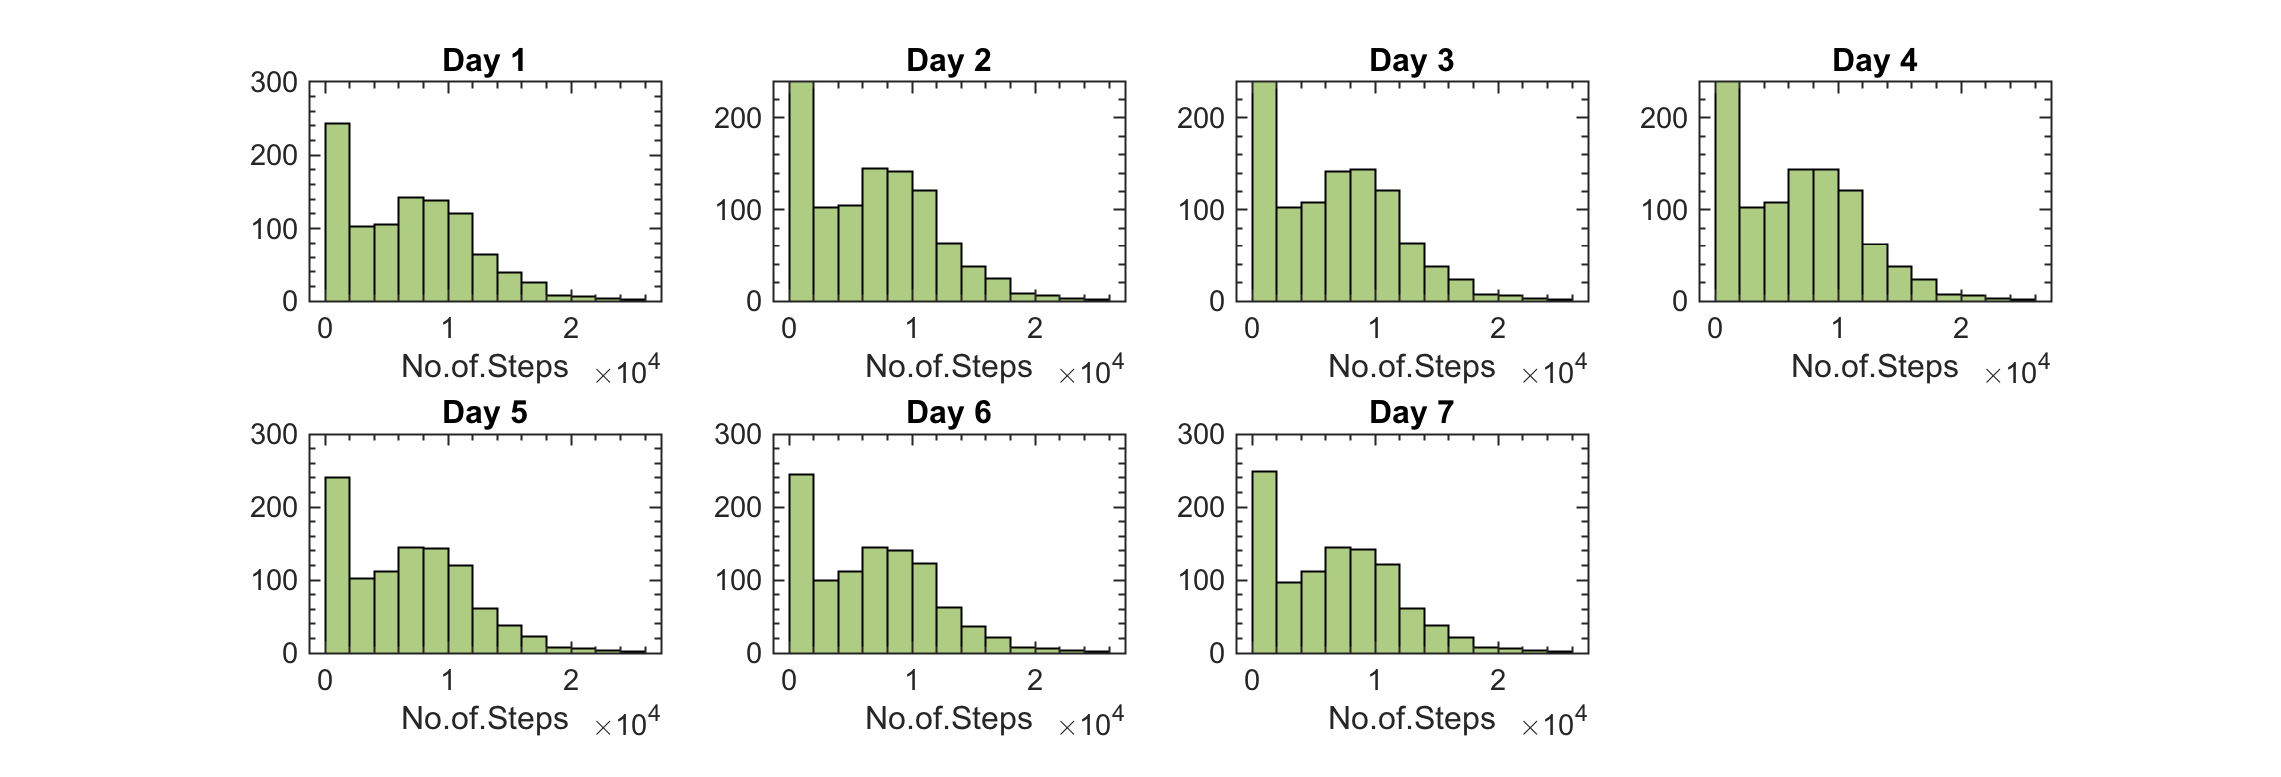
\includegraphics[width=1.1\linewidth]{7dayhist.eps}
    \caption{Daily Steps Distribution}
  \label{fig:4}
\end{figure}

\subsubsection{Shannon Entropy}
In addition we compute the Shannon entropy \cite{shannon1948mathematical} for the aforementioned feature vector using the equation below.


\begin{equation}
   H(x) = -\sum_{i=1}^{7}p_{i}\ln(p_{i})
\end{equation}
where $i$ denotes the day, and $H(x)$ denotes the normalized Shannon entropy of the seven daily step counts monitored during the seven days of a week. The normalized Shannon entropy varies between 0 and 1. A value close to zero indicates that the step counts of the participant through the week are irregular; in contrast, a value close one indicates that the step counts are consistent over the week. In total there are 26 (=18+7+1) candidate predictors for building the machine learning model.  


\subsubsection{Random Forest}
Random forests (RF) are chiefly used for building predictive models, for both classification and regression problems. The RF can be interpreted easily and are less susceptible to underfitting \citep{genuer2010variable}. The other application of RF is to aid feature selection. The RF generate a series of uncorrelated decision trees and finally funnels into best possible solution. For screening features, the ones at the top of the trees are considered more important than those at end of the tree.
\par
In this work the 26 candidate predictors are further screened using RF approach \cite{genuer2010variable}. In the RF based approach, we ran the training process in two nested loops to select the optimal size and composition of the predictor variable set. In the inner loop we create 100 different trees. Each tree is trained with out-of-bag samples with replacement from the training data set and is terminated when the number of decision variables (decision nodes) in the tree exceeds a threshold $k$, where $k = 1, 2, ..., 26$. Then the decision variables are selected considering the frequency with which they appear in the 100 trees. The more frequently appearing variables are preferentially selected over the less frequently appearing variables. This process identifies variables that are invariant to the training dataset composition and eliminates the ones that are sensitive to the composition of the training dataset. The activity in the inner loop identifies the set of predictors variables when the set size is $k$. The outer loop is used to determine the optimum value of $k$, which computes average RMSE (root mean squared error) for each $k$, through 10-fold cross validation approach. The outer loop is repeated 10 times. The RMSE of 100 trees with $k$-decision variables and 10 fold validation are averaged. Table [\ref{tab:RF_RMSE}] in supplementary material gives the average RMSE for each $k$. Using these results, we built a RMSE versus $k$ plot as shown in Figure [\ref{fig:5}]. The plot indicates that $k$=5 yields the minimum average RMSE with 66\% of total variance explained. The importance of variables in RF is shown in Figure [\ref{fig:6}]. Five variables are found to be important in the following order: Entropy, Factor 16, Factor 2, Factor 7 and Factor 10. In total there are 5 predictors for building the machine learning model. We reported top 10 important variables based on their associated loading with each factor in supplementary materials [\ref{fig:8},\ref{fig:9},\ref{fig:10},\ref{fig:11}]

\begin{figure}%[H]
\begin{minipage}{0.5\textwidth}
\includegraphics[width=1\linewidth]{RF_L_CHART_FINAL.png}
\noindent\caption{Selection of number of variables using RF} 
\label{fig:5}
\end{minipage}
\begin{minipage}{0.5\textwidth}
\noindent\includegraphics[width=1\linewidth]{RF_Importance_FINAL.png}
\caption{Important variable selection using RF} 
\label{fig:6}
\end{minipage}
\end{figure}


In the knowledge-based approach we select the two most relevant variables that we found in our previous study of factors influencing exercise engagement among people using activity trackers [Ramin's previous ref]. These two factors are (1) how many technological devices the participant own, and (2) if members of the participant’s family use activity fitness trackers and other smart devices. To these two predictors we add step count for each of the past 7 days of the week and the normalized Shannon entropy  of the 7 step counts. In total there are 10 (=2+7+1) predictors for building the machine learning model.

\subsection{Model Development}
To choose an appropriate machine learning models we compare a linear model (regularized linear regression) vs a non-linear model (regularized feed forward neural networks). We trained the linear and the non-linear models over the training dataset using 10-fold cross validation for 10 replications. We perform the t-test comparison between Neural network model and linear regression model predictions over the test dataset. The null hypothesis for t-test was that the error mean between two models are the same with the alternative hypothesis that the neural network model has lower mean error than the linear model. We reject the null hypothesis with p-value of $2.2 {e^{-16}}$. We also reported R-square, RMSE and MAE in supplementary materials [\ref{tab:Performance_linear_neuralnet}, \ref{fig:12}]. Rather than searching between different non-linear models we focus on exploring different neural network architectures to find an optimal one. Two neural network models were developed, one for each variable selection method. For each neural network model we used ad-hoc search to find the optimal number of hidden nodes for each layer as shown in Supplementary Material [\ref{tab:DDNN}, \ref{tab:KBNN}]. Each model was run with 10-fold cross validation for 3 replications with a learning rate of $0.0001$. The optimal number of hidden units in each layer are found using R-squared and RMSE.

\begin{figure}[t]
\centering
   \begin{subfigure}{0.48\linewidth} \centering
     \includegraphics[scale=0.42]{DDNN_17042019.png}
     \vspace*{-20mm}
     \caption{DDNN}\label{fig:figA}
   \end{subfigure}
   \begin{subfigure}{0.48\linewidth} \centering
     \includegraphics[scale=0.42]{KKNN.png}
     \vspace*{-20mm}
     \caption{KBNN}\label{fig:figB}
   \end{subfigure}
\caption{Neural networks architecture} \label{fig:twofigs}
\label{fig:7}
\end{figure}

\subsubsection{Model 1: Neural Network based on Data Driven variables (DDNN)}
The neural network architecture includes five input nodes and three hidden layers, each with 4 hidden nodes Figure [\ref{fig:7}]. The black lines indicate positive weights on the connections and the grey lines indicate negative weights. The line thickness is proportional to magnitude of the weight of the connection. Each of the five variables are shown as inputs to the first layer  $\{x_i\}^{5} _{i:1}$ labelled with xi. The response variable is shown in the far-right layer (labelled Y). The input nodes are labeled $\{I_i\}^{5} _{i:1}$ and hidden nodes are labelled $\{H_i\}^{4} _{i:1}$ for each hidden layer with $\{B_i\}^{4} _{i:1}$ as bias nodes. 
\subsubsection{Model 2: Neural Network based on Knowledge based variables (KBNN)}
The neural network was developed using 10 input variables $\{x_i\}^{10} _{i:1}$ and three hidden layers with 3 hidden units in each layer [Figure \ref{fig:7}]. Just as in the data-driven neural network model, black lines in the knowledge-based neural network are positive weights and the grey lines are negative weights. The hidden nodes are labelled as $\{H_i\}^{3} _{i:1}$ for each hidden layer with $\{B_i\}^{3} _{i:1}$ as bias nodes.

To compare the performances of the models, we used RMSE and R-Squared value reported in Table [\ref{tab:Performance}] and Figure [\ref{fig:2}].

\subsection{Data analysis pipeline}
In summary, the Wellocaracy algorithm consists of the following steps:

1. Create a dataset of 20 participants as a matrix n of size 20\x94

2. Generate a dataseet combining weekly steps per participants and feature extracted from factor analysis and Shannon entropy.

3. Train two neural network models, one for data derived automatically from random forest model and the other for knowledge discovered from authors' previous work.

4. Compare both DDNN and KBNN model. 

All steps are shown in Figure [\ref{fig:1}].

\section{Study Limitation \& Future Work}
This study had a few limitations. Target enrollment was low, and all participants
were recruited from the same lab, which may limit the generalizability of the
study. Additionally, a larger n may have resulted in more significant results.
PRTICIPANTS who choose to be in this study may more liklely to be engaged with FITBIT trackers compared to those who chose not to participate in the study.
\par
As a extension to the current work, a new study with the goal of validation of the model has been undertaken with an IRB approval. The new study recruited 120 individuals from the general public to use the DDNN model over a period of 6 months. The DDNN model has been deployed on a (\url{http://wellocracystudy.org}) server as a backend for new participants. Each participant received a FitBit activity tracker device. the DDNN model predicts a weekly target value for a given participant and update the model parameters on a weekly basis with regard to the participants performance over the week. 



\section{Code Availability}
The code used for this analysis is available upon reasonable request but it
is not publicly available. Requests to access the codes will be reviewed by
the project PI to verify whether restrictions due to Intellectual
Property apply.

\section{Data Availability}
The data that support the findings of this study are available upon reasonable
request.

\section{Protocols}

\section{Acknowledgment}
This research was supported in conjunction with a grant from the Robert Wood Johnson Foundation (Grant ID: 71963).


\section{Author Contribution}
Mohammadi.R and Kamarthi.S worked on data exploration, dimension reduction through factor analysis, and implementing and designing neural network based algorithm and generating results and preparing the draft of the paper. He is one of the guarantor authors of the paper.


\bibliographystyle{model1-num-names}
\bibliography{sample.bib}
\newpage
\section{Supplementary Material}


\begin{table}[H]
\centering
\caption{Random forest resampling performance}
\begin{tabular}{llllll}
\hline
\# of Variables & RMSE     & R-squared & \# of Variables & RMSE     & R-squared \\
\hline
1               & 1857.509 & 0.65068   & 14              & 1854.075 & 0.65027   \\
2               & 1853.287 & 0.65174   & 15              & 1855.636 & 0.64952   \\
3               & 1842.335 & 0.65576   & 16              & 1857.846 & 0.64902   \\
4               & 1835.522 & 0.65774   & 17              & 1859.988 & 0.64816   \\
5               & 1834.349 & 0.65811   & 18              & 1866.535 & 0.64567   \\
6               & 1835.721 & 0.65733   & 19              & 1867.687 & 0.64533   \\
7               & 1839.676 & 0.6559    & 20              & 1869.874 & 0.64444   \\
8               & 1837.493 & 0.65691   & 21              & 1868.629 & 0.64495   \\
9               & 1838.974 & 0.65597   & 22              & 1877.417 & 0.6418    \\
10              & 1841.605 & 0.65502   & 23              & 1876.553 & 0.64203   \\
11              & 1846.311 & 0.65348   & 24              & 1879.596 & 0.64099   \\
12              & 1848.945 & 0.65218   & 25              & 1879.082 & 0.64102   \\
13              & 1853.418 & 0.65059   & 26              & 1880.87  & 0.64065 \\
\hline
\label{tab:RF_RMSE}
\end{tabular}
\end{table}

\begin{table}[H]
\centering
\caption{Data Driven Neural Network Resampling Performance}
\begin{tabular}{lllllll}
\hline
Sno & Layer1 & Layer2 & Layer3 & RMSE & R-Squared &        \\
\hline
1      & 2      & 2      & 2    & 24.6178   & 0.5226 \\
2      & 3      & 3      & 3    & 26.479    & 0.5999 \\
3      & 4      & 4      & 4    & 25.3374   & 0.6946 \\
4      & 5      & 5      & 5    & 41.7103   & 0.619 \\
\hline
\label{tab:DDNN}
\end{tabular}
\end{table}


\begin{table}[H]
\centering
\caption{Knowledge Based Neural Network Resampling Performance}

\begin{tabular}{lllllll}
\hline
Sno & layer1 & layer2 & Layer3 & RMSE     & R-Squared \\
\hline
1   & 3      & 3      & 3      & 2307.495 & 0.4629    \\
2   & 4      & 4      & 4      & 2342.624 & 0.4711    \\
3   & 5      & 5      & 5      & 2464.502 & 0.4339    \\
4   & 6      & 6      & 6      & 7133.92  & 0.3443    \\
5   & 7      & 7      & 7      & 2976.689 & 0.3302    \\
6   & 8      & 8      & 8      & 4870.065 & 0.3027   \\
\hline
\label{tab:KBNN}
\end{tabular}
\end{table}

\newpage
\begin{table}[H]
\centering
\caption{DDNN variable names}
\begin{tabular}{llll}
\hline
Variable  & Variable name & Variable    & Variable name \\
\hline
Factor 1  & x1           & Factor 15   & x15            \\
Factor 2  & x2           & Factor 16   & x16            \\
Factor 3  & x3           & Factor 17   & x17           \\
Factor 4  & x4           & Factor 18   & x18           \\
Factor 5  & x5           & Day 1 steps & x19           \\
Factor 6  & x6           & Day 2 steps & x20           \\
Factor 7  & x7           & Day 3 steps & x21           \\
Factor 8  & x8           & Day 4 steps & x22           \\
Factor 9  & x9           & Day 5 steps & x23           \\
Factor 10 & x10          & Day 6 steps & x24           \\
Factor 11 & x11          & Day 7 steps & x25         \\
Factor 12 & x12          & Entropy & x26           \\
Factor 13 & x13          & Target &  Y   \\
Factor 14 & x14          &            \\
\hline
\label{tab:DDNN_Variable_names}
\end{tabular}
\end{table}

\begin{table}[H]
\centering
\caption{KBNN variable names}
\begin{tabular}{llll}
\hline
Variable      & Variable name & Variable    & Variable name \\
\hline
Entropy       & x1            & Day 4 steps & x7            \\
Owned Tech    & x2            & Day 5 steps & x8            \\
Friends Track & x3            & Day 6 steps & x9            \\
Day 1 steps   & x4            & Day 7 steps & x10           \\
Day 2 steps   & x5            & Target      & Y             \\
Day 3 steps   & x6            &             &           \\
\hline
\label{tab:KBNN_Variable_names}
\end{tabular}
\end{table}

\begin{figure}[H]
\centering
  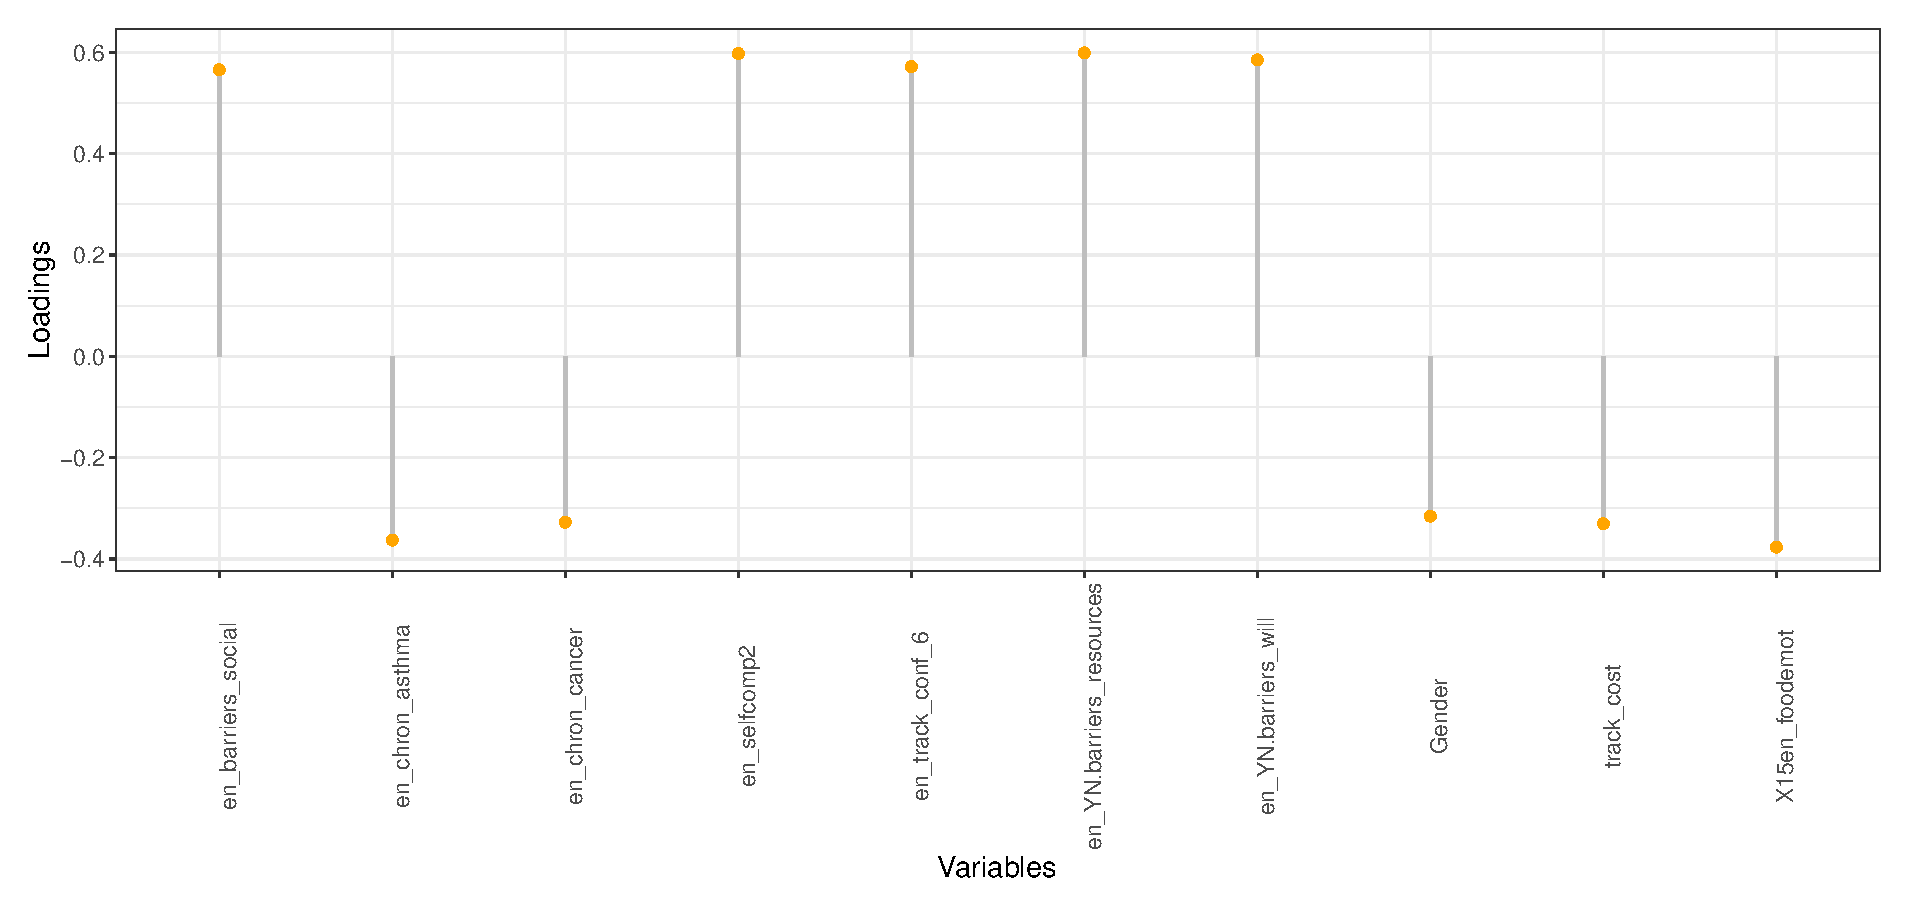
\includegraphics[width=1\linewidth]{factorMR2.eps}
  \caption{Loadings for factor MR2}
  \label{fig:8}
\end{figure}
\begin{figure}[H]
\centering
  \includegraphics[width=1\linewidth]{factorMR6.eps}
    \caption{Loadings for factor MR6}
  \label{fig:9}
\end{figure}
\begin{figure}[H]
\centering
  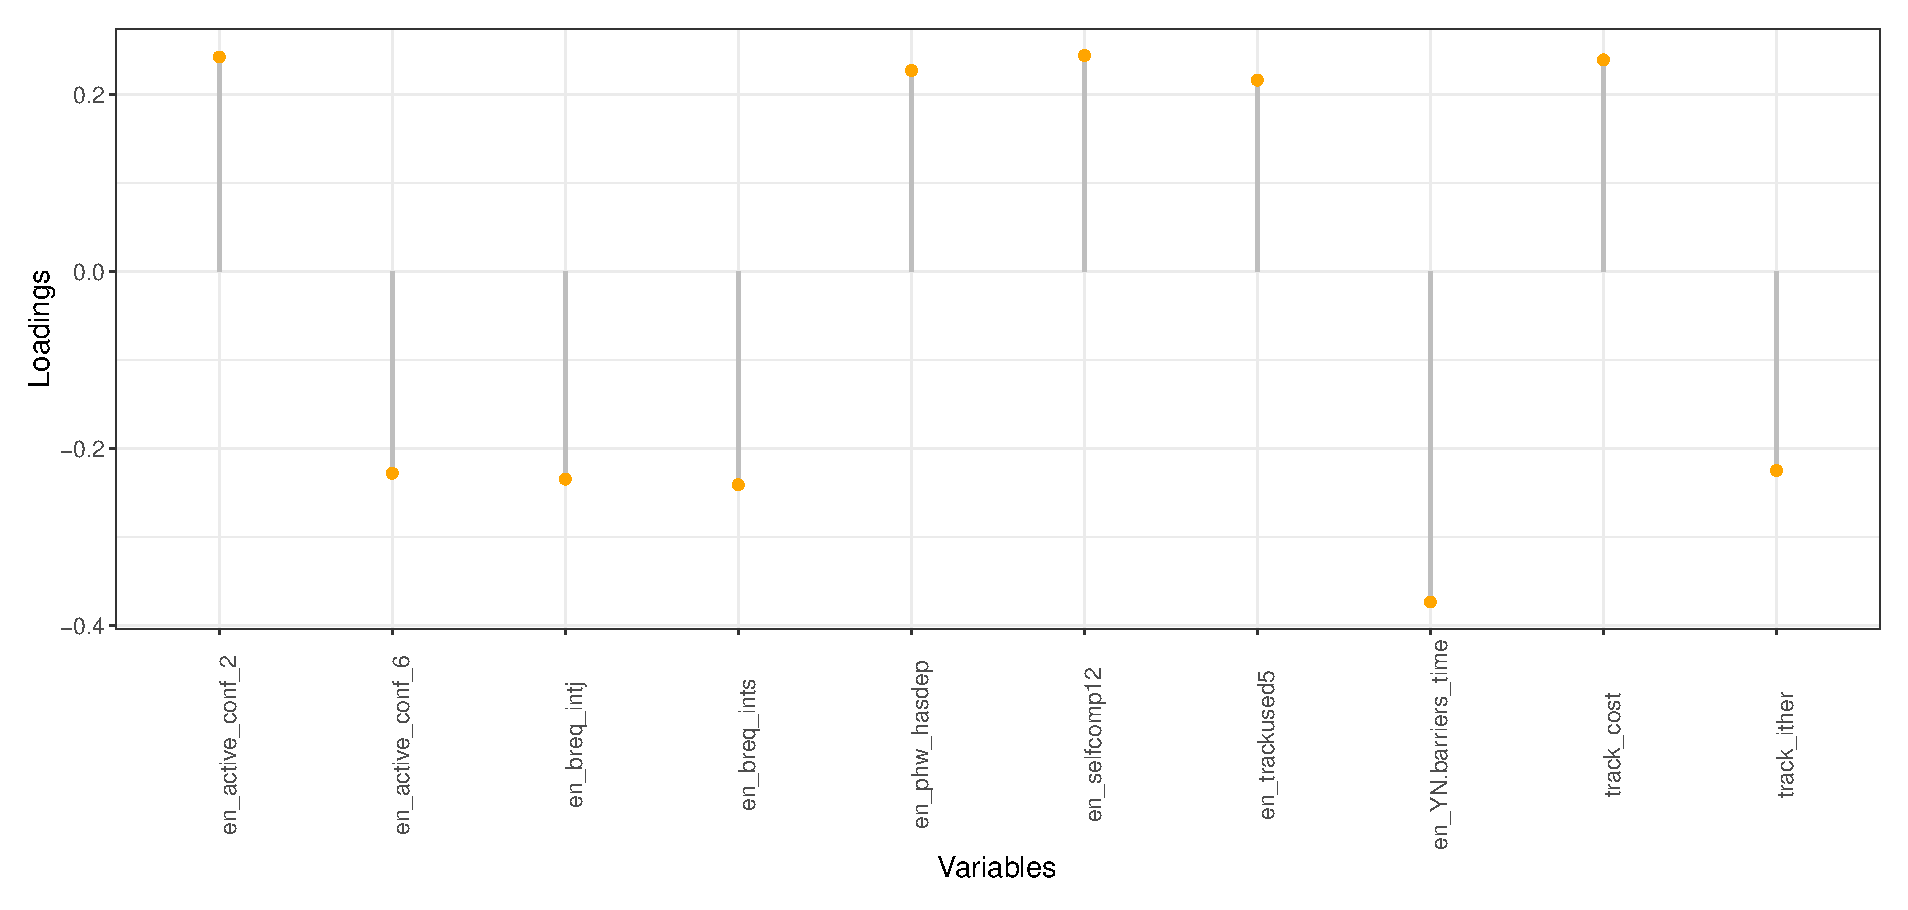
\includegraphics[width=1\linewidth]{factorMR16.eps}
    \caption{Loadings for factor MR16}
  \label{fig:10}
\end{figure}
\begin{figure}[H]
\centering
  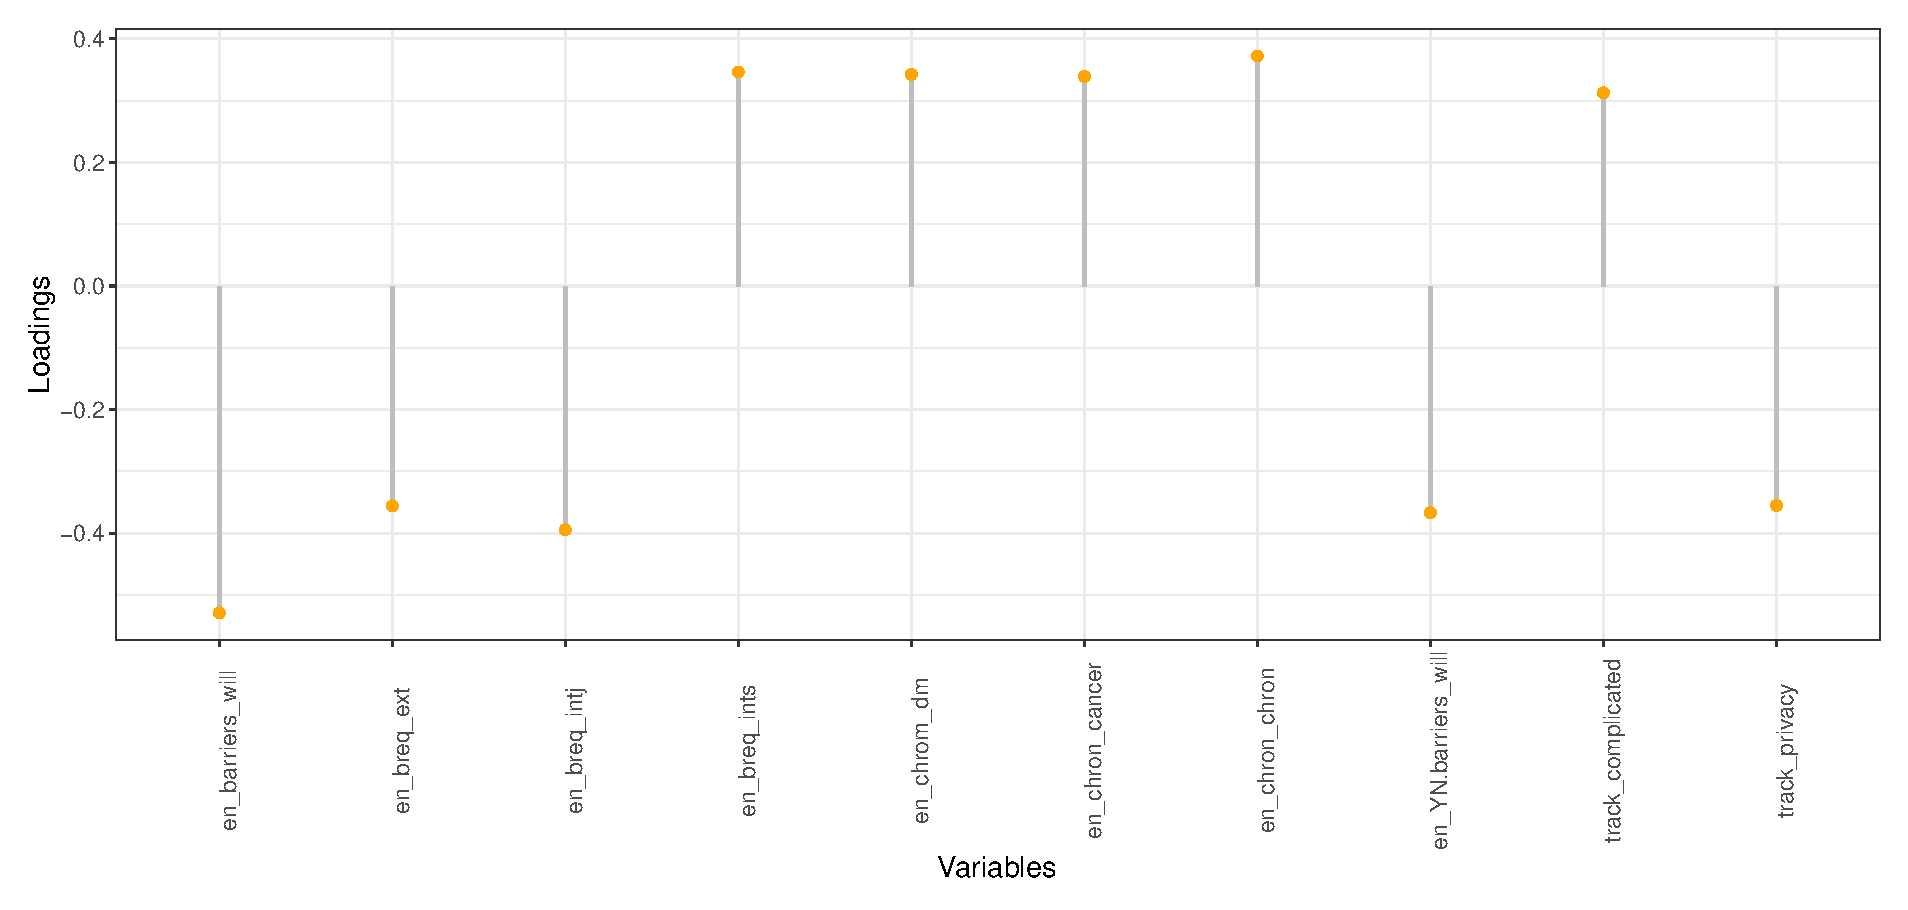
\includegraphics[width=1\linewidth]{factorMR7.eps}
    \caption{Loadings for factor MR7}
  \label{fig:11}
\end{figure}

\begin{table}[H]
\centering
\caption{Models perfromance comparison}
\begin{tabular}{l|l|l|l}
\textbf{MAE}                   & \textbf{Min.} & \textbf{Median} & \textbf{Mean} \\ \hline
\textbf{Linear Regression}     & 2040.60       & 2246.17         & 2247.26       \\ \cline{2-4} 
\textbf{Vaniala Neural Network} & 1680.94       & 1958.40         & 1950.67       \\ \hline
\textbf{RMSE}                  & \textbf{Min.} & \textbf{Median} & \textbf{Mean} \\ \hline
\textbf{Linear Regression}     & 2463.97       & 2776.59         & 2800.21       \\ \cline{2-4} 
\textbf{Vaniala Neural Network} & 2155.12       & 2556.90         & 2515.33      
\label{tab:Performance_linear_neuralnet}
\end{tabular}
\end{table}


\begin{figure}[H]
\centering
  \includegraphics[width=1.1\linewidth]{LR_NN_Comparision_04182019.png}
    \caption{Daily Steps Distribution}
  \label{fig:12}
\end{figure}


%% main text

%% The Appendices part is started with the command \appendix;
%% appendix sections are then done as normal sections
%% \appendix

%% \section{}
%% \label{}

%% References
%%
%% Following citation commands can be used in the body text:
%% Usage of \cite is as follows:
%%   \cite{key}          ==>>  [#]
%%   \cite[chap. 2]{key} ==>>  [#, chap. 2]
%%   \citet{key}         ==>>  Author [#]

%% References with bibTeX database:



%% Authors are advised to submit their bibtex database files. They are
%% requested to list a bibtex style file in the manuscript if they do
%% not want to use model1-num-names.bst.

%% References without bibTeX database:

% \begin{thebibliography}{00}

%% \bibitem must have the following form:
%%   \bibitem{key}...
%%

% \bibitem{}

% \end{thebibliography}


\end{document}

%%
%% End of file `elsarticle-template-1-num.tex'.